\documentclass[preprint]{transcrypto}

%%%% 2. PACKAGES %%%%
\usepackage{lipsum} % Example package -- can be removed
\usepackage{tikz}
\usepackage{graphicx}
\usepackage{subcaption}
\usepackage[noend]{algorithmic}
\usepackage{float}
\usepackage{amsmath}
\usepackage{enumitem}
\usepackage[utf8]{inputenc}
\usepackage[english]{babel}
\usepackage[backend=biber,style=numeric,sorting=ynt]{biblatex}
\renewbibmacro{in:}{}
\addbibresource{sample.bib}
\usetikzlibrary{shapes,arrows,positioning,calc}
\usetikzlibrary{decorations.pathreplacing}
% ---------------------------------
\makeatletter
\newcommand*{\rectxy@anchor@top}[2]{%
  \anchor{t#1}{%
    \pgf@process{\southwest}%
    \pgf@xa=\pgf@x
    \pgf@process{\northeast}%
    \pgf@x=\dimexpr\pgf@xa + (\pgf@x-\pgf@xa)*#1/#2\relax
  }%
}
\newcommand*{\rectxy@anchor@bottom}[2]{%
  \anchor{b#1}{%
    \pgf@process{\northeast}%
    \pgf@xa=\pgf@x
    \pgf@process{\southwest}%
    \pgf@x=\dimexpr\pgf@x + (\pgf@xa-\pgf@x)*#1/#2\relax
  }%
}
\newcommand*{\rectxy@anchor@left}[2]{%
  \anchor{l#1}{%
    \pgf@process{\northeast}%
    \pgf@ya=\pgf@y
    \pgf@process{\southwest}%
    \pgf@y=\dimexpr\pgf@y + (\pgf@ya-\pgf@y)*#1/#2\relax
  }%
}
\newcommand*{\rectxy@anchor@right}[2]{%
  \anchor{r#1}{%
    \pgf@process{\southwest}%
    \pgf@ya=\pgf@y
    \pgf@process{\northeast}%
    \pgf@y=\dimexpr\pgf@ya + (\pgf@y-\pgf@ya)*#1/#2\relax
  }%
}
\newcommand*{\declareshaperectxy}[2]{%
  \pgfdeclareshape{rectangle #1x#2}{%
    \inheritsavedanchors[from=rectangle]
    \inheritanchorborder[from=rectangle]
    \inheritanchor[from=rectangle]{north}
    \inheritanchor[from=rectangle]{north west}
    \inheritanchor[from=rectangle]{center}
    \inheritanchor[from=rectangle]{west}
    \inheritanchor[from=rectangle]{east}
    \inheritanchor[from=rectangle]{mid}
    \inheritanchor[from=rectangle]{mid west}
    \inheritanchor[from=rectangle]{mid east}
    \inheritanchor[from=rectangle]{base}
    \inheritanchor[from=rectangle]{base west}
    \inheritanchor[from=rectangle]{base east}
    \inheritanchor[from=rectangle]{south}
    \inheritanchor[from=rectangle]{south east}
    \inheritbackgroundpath[from=rectangle]
    \count@=\m@ne
    \@whilenum\count@<#1 \do{%
      \advance\count@\@ne
      \expandafter\rectxy@anchor@top\expandafter{\the\count@}{#1}%
      \expandafter\rectxy@anchor@bottom\expandafter{\the\count@}{#1}%
    }%
    \count@=\m@ne
    \@whilenum\count@<#2 \do{%
      \advance\count@\@ne
      \expandafter\rectxy@anchor@left\expandafter{\the\count@}{#2}%
      \expandafter\rectxy@anchor@right\expandafter{\the\count@}{#2}%
    }%
  }%
}
\makeatother

\declareshaperectxy{16}{8}
\declareshaperectxy{5}{3}
\declareshaperectxy{3}{0}

% ------------------------------------------------------

%%%% 3. AUTHOR, INSTITUTE %%%%
\author{Abhishek Shingane\inst{1}, Gopal Ramesh Dahale\inst{2} \and Kumari Rani\inst{3}}
\institute{
  11840040, IIT Bhilai, \email{abhisheks@iitbhilai.ac.in}
  \and
  11840520, IIT Bhilai, \email{gopald@iitbhilai.ac.in}
  \and
  11840690, IIT Bhilai, \email{krani@iitbhilai.ac.in}\
}
%%%% NOTES:
% - We need a city name for indexation purpose, even if it is redundant
%   (eg: University of Atlantis, Atlantis, Atlantis)
% - \inst{} can be omitted if there is a single institute,
%   or exactly one institute per author

%%%% 4. TITLE %%%%
\title{PRESENT Cipher}
%%%% NOTES:
% - If the title is too long, or includes special macro, please
%   provide a "running title" as optional argument: \title[Short]{Long}
% - You can provide an optional subtitle with \subtitle.

\begin{document}
\maketitle

%%%% 5. KEYWORDS %%%%
\keywords{PRESENT \and Differential cryptanalysis \and Linear Cryptanalysis \and Correlation Analysis}

%%%% 6. ABSTRACT %%%%
\begin{abstract}
  In this paper we focus on the Present Cipher. We describe the design of the Cipher and comment on the design decisions taken while developing the cipher. We then discuss two popular cryptanalysis namely Differential cryptanalysis  and Linear cryptanalysis on round reduced version of the Cipher. We also discuss an interesting experiment and show that the run-time of cipher does not have any co-relation with number of bits high in key.
\end{abstract}

%%%% 7. PAPER CONTENT %%%%
\section{Introduction}
% Widely used primitives like the AES~\cite{AES} do not have perfect
% security, and can be analysed with linear
% cryptanalysis~\cite{EC:Matsui93}, differential
% cryptanalysis~\cite{JC:BihSha91}, or differential power
% analysis~\cite{C:KocJafJun99}.  We show that the One-Time-Pad is
% unconditionally secure in \autoref{sec:main}.
% \section{Main Result}
% \label{sec:main}
% \lipsum
Advanced Encryption Standard(AES) and Data Encryption Standard (DES) are the most studied algorithms in cryptanalysis, other than the limitations of key length in DES, both the algorithms have proven resistance against various cryptanalysis techniques developed to compromise the security of ciphers. Similar to AES and DES, the Present cipher is a block cipher. The structure of the Present is distinctly similar to AES. But unlike AES and DES, the Present cipher is a lightweight cipher designed with the goal of hardware performance on low powered devices while providing reasonable security. The Present cipher is now ISO/IEC 29192-2:2019 standard. The cipher is majorly used in applications with low computing power like RFID cards or IoT nodes. Similar to AES the round reduced versions are vulnerable to various cryptanalysis techniques including Linear and Differential cryptanalysis.


\section{List of contributions : }
\begin{enumerate}
    \item Gopal Ramesh Dahale : Gopal analysed the design choices of the PRESENT cipher. He examined the properties of the S-box and the permutation layer, which ensured that the cipher is resistant to various attacks. He studied and analysed the specifications of the cipher and he also implemented the cipher in python. 
    \item Abhishek Shingane : Abhishek implemented the differential attack on the 3-rounds of the PRESENT cipher in python using the idea of differential and filtering. He also proposed an experiment to find some correlation between the key and the time taken by the encryption function.
    \item Kumari Rani : Rani analysed the differential properties of the PRESENT cipher and did a theoretical attack on 16-rounds of PRESENT cipher. She also analysed the resistance of the cipher against linear attacks. 
    
\end{enumerate}

\section{The Present Cipher \textsuperscript{\cite{5}}}
The Present cipher is an Ultra-Lightweight block cipher. The cipher has a block length of 64 bits and supports 80-bit and 128-bit keys. We describe and analyze the 80-bit version of Present cipher as security provided by an 80-bit key is adequate for applications like RFID tags and IoT security and the security claims of 128-bit version is added in the appendix. The present cipher has a public S-box, Bit Permutation, and key schedule.
\\
% the credit of below diagram goes to iacr.org/authors/tikz/
\begin{figure}[H]
    \centering
    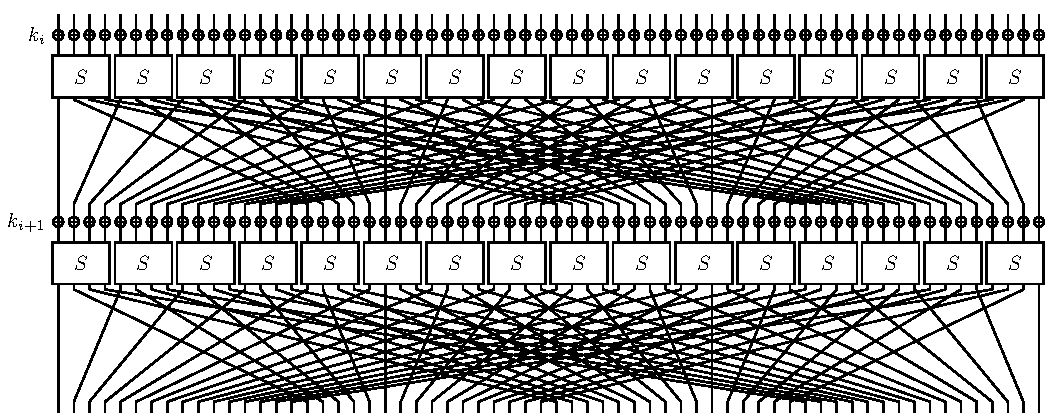
\includegraphics[width=\linewidth]{PRESENT_diagram.pdf}
    \caption{SP Network for Present Cipher \textsuperscript{\cite{5}}}
\end{figure}

\subsection{Cipher Design}
The Present-80 is an example of SP-network, with 31 rounds. Each round consists of a xor of the round key followed by 4-bit non-linear substitution layer and linear bit-wise permutation. The 4-bit S-Box is applied 16 times in parallel for the 64-bit input during each round. \figurename .{\ref{fig:top-level} \subref{fig:pseudocode}} shows the higher level pseudo-code for implementing the encryption algorithm. \figurename .{\ref{fig:top-level} \subref{fig:top-level-diagram}} is a top-level description of the encryption algorithm.

\tikzset{
    block/.style = {
        draw, 
        fill=white, 
        rectangle, 
        minimum height=1.8em, 
        minimum width = 10em
    },
    block2/.style = {
        draw, 
        fill=white, 
        rectangle, 
        minimum height=3.7em, 
        minimum width=6em
    },
    sum/.style = {
        draw, 
        fill=white, 
        circle, 
        inner sep=0pt,
        minimum size = 0.5cm
    },
    pinstyle/.style = {
        pin edge={to-,thin,black}
    }
}

\begin{figure}[h!]
    \captionof{figure}{A top-level algorithmic description of present}\label{fig:top-level}
    \centering
    \begin{subfigure}[b]{0.3\linewidth}
        \begin{algorithmic}
            \STATE{generateRoundKeys()}
            \FOR{$i=1$ \TO $31$ }
                \STATE {addRoundKey(\textsc{State},$K_i$)} 
                \STATE {sBoxLayer(\textsc{State})} 
                \STATE {pLayer(\textsc{State})} 
            \ENDFOR
            \STATE addRoundKey(\textsc{State},$K_{32}$)
        \end{algorithmic}
        \caption{}
        \label{fig:pseudocode}
    \end{subfigure}
    \hspace{60pt}
    \begin{subfigure}[b]{0.5\linewidth}
        \begin{tikzpicture}[auto, node distance=2cm,>=latex',scale=0.6, every node/.style={scale=0.6}]
            % nodes
            \node [sum] (sum1) {+};
            \node [block,above of=sum1,node distance=1cm] (plaintext) {plaintext};
            \node [block,right of=plaintext,node distance=5cm] (keyregister) {key register};
            \node [block,below of=sum1,node distance=1cm] (sBoxLayer) {sBoxLayer};
            \node [block,below of=sBoxLayer,node distance=0.7cm] (pLayer) {pLayer};
            \node [block,below of=pLayer,node distance=4cm] (sBoxLayer2) {sBoxLayer};
            \node [block,below of=sBoxLayer2,node distance=0.7cm] (pLayer2) {pLayer};
            \node [sum, below of=pLayer2,node distance=1cm] (sum2) {+};
            \node [block,below of=sum2,node distance=1cm] (ciphertext) {ciphertext};
            
            \node [block2,below of=keyregister,node distance=2.35cm] (update) {update};
            \node [block2,below of=update,node distance=4.7cm] (update2) {update};
        
            % arrows
            \draw [->] (plaintext) -- (sum1);
            \draw [->] (sum1) -- (sBoxLayer);
            \draw [->] (pLayer2) -- (sum2);
            \draw [->] (sum2) -- (ciphertext);
            \draw [->] (keyregister) -- (update);
            \draw [->,dashed] (update) -- (update2);
            \draw [->,dashed] (pLayer) -- (sBoxLayer2);
            \draw [->] (keyregister)  |- node[above left= 0pt] {addRoundKey            }    (sum1);
            \draw [->] (update2) |- node[above left= 0pt]{addRoundKey            }   (sum2);
        \end{tikzpicture}
        \caption{} 
        \label{fig:top-level-diagram}
    \end{subfigure}
  
  \end{figure}
  
\subsection{Add Round Key}
Provided the round key $K_i = k_{63},k_{62} \dots k_0$ for $1\leq i \leq 32$ and the current state $S = s_{63},s_{62}\dots s_0$, addRoundKey performs the following operation
\begin{eqnarray*}
    S \xrightarrow{} S \oplus K_i \\
    \implies s_t \xrightarrow[]{} s_t \oplus k_t 
\end{eqnarray*}
for $0\leq t\leq 63$.

\subsection{Substitution Layer}
The substitution box is 4-bit to 4-bit mapping. Table \ref{pSbox} shows the mapping of S-Box in Hexadecimal notation. The 4-bit S-Box is independently repeated 16 times to cover the 64-bit block.
\begin{figure}[h!]
    \centering
    \begin{tabular}{ |c||c|c|c|c|c|c|c|c|c|c|c|c|c|c|c|c| }
        \hline
        $x$ & 0 & 1 & 2 & 3&4& 5& 6&7&8&9&A&B&C&D&E&F  \\ \hline
        $S[x]$& C & 5 & 6& B &9 &0 &A &D& 3& E &F& 8& 4 &7& 1& 2 \\ \hline
    \end{tabular}
    \captionof{table}{Present sBox}\label{pSbox}
\end{figure}
The substitution box is a mapping $S:\mathbb{F}_2^4\xrightarrow[]{}\mathbb{F}_2^4$ where $\mathbb{F}$ is a finite field. To improve the avalanche-effect, the PRESENT S-Box satisfies the following conditions.

First, denote the Fourier coefficient of the S-Box by
\begin{equation}
    S_b^W (a) = \sum_{x \in \mathbb{F}_2^4} (-1)^{\langle b,S(x)\rangle + \langle a,x\rangle}
\end{equation}
\begin{enumerate}
    \item For any fixed input difference $\Delta_I \in \mathbb{F}_2^4,\Delta_I \not = 0$ and output difference $\Delta_O \in \mathbb{F}_2^4,\Delta_I \not = 0$, the following condition must be satisfied
    \begin{equation*}
        |\{ x \in \mathbb{F}_2^4~~ \vert~~ S(\Delta_I +x) + S(x) = \Delta_O \}| \leq 4
    \end{equation*}
    \item For any fixed input difference $\Delta_I \in \mathbb{F}_2^4,\Delta_I \not = 0$ and output difference $\Delta_O \in \mathbb{F}_2^4$ such that $wt(\Delta_O) = wt(\Delta_I) = 1$, the following condition must be satisfied
    \begin{equation*}
        \{ x \in \mathbb{F}_2^4~~ \vert~~  S(\Delta_I +x) + S(x) = \Delta_O  \} = \Phi
    \end{equation*}
    where $wt(x)$ is the hamming weight of $x$.
    \item For all $a \in \mathbb{F}_2^4, a \not = 0 $ and $b \in \mathbb{F}_4$, $|S_b^W (a)| \leq 8$ holds.
    \item For all $a \in \mathbb{F}_2^4, a \not = 0 $ and $b \in \mathbb{F}_4$ such that $wt(b) = wt(a) = 1$, $S_b^W (a) = \pm 4 $ holds.
\end{enumerate}
\subsection{Permutation Layer} 
The permutation layer is a bit permutation. The permutation function P(i) maps the $i^{th}$ bit of input to P(i) in the output of the permutation layer. The Table {\ref{pLayer}} is the mapping of P(i) in tabular form. Fig.5 shows the visual representation of the Add round key, Substitution layer, and Permutation layer for one round.
\begin{figure}[h!]
    \centering
    \begin{tabular}{ |c||c|c|c|c|c|c|c|c|c|c|c|c|c|c|c|c| }
        \hline
        i& 0 &1 &2 &3& 4& 5& 6 &7 &8 &9 &10 &11 &12 &13 &14 &15 \\
        P(i) &0& 16& 32& 48& 1& 17& 33&49& 2 &18& 34& 50& 3 &19 &35 &51 \\\hline\hline
        i &16& 17& 18& 19& 20& 21 &22& 23 &24 &25 &26 &27 &28 &29 &30 &31 \\
        P(i)& 4 &20 &36& 52& 5& 21 &37& 53& 6 &22& 38& 54& 7 &23 &39 &55 \\\hline\hline
        i &32& 33& 34& 35& 36& 37 &38& 39 &40 &41 &42 &43 &44 &45 &46 &47 \\
        P(i) &8 &24& 40& 56 &9& 25 &41 &57 &10 &26 &42 &58 &11 &27 &43 &59 \\\hline\hline
        i &48& 49& 50 &51 &52 &53& 54& 55 &56 &57 &58 &59 &60 &61 &62 &63 \\
        P(i) &12& 28& 44&60& 13 &29& 45& 61 &14 &30 &46 &62 &15 &31 &47 &63 \\\hline
    \end{tabular}
    \captionof{table}{Present pLayer}\label{pLayer}
\end{figure}
\subsection{Key schedule Algorithm}
The Present cipher supports 80-bit or 128-bit long key, in this section we discuss the 80-bit key schedule algorithm. Firstly, the initial 80-bit key is stored in a key register $K$ and is represented as $K = k_{79}k_{78}$..$k_0$. At any round $i$, PRESENT extracts the 64-bits round key $K_i = \mathrm{k_{63}}\mathrm{k_{62}}$..$\mathrm{k_{0s}}$ from the current Key (left most 64 bits) register as follows : 
\begin{equation*}
    K_i = \mathrm{k_{63}}\mathrm{k_{62}}..\mathrm{k_{0s}} = k_{79}k_{78}..k_{16}
\end{equation*}
After round key extraction, the key register $K$ is updated according to the following rules : 
\begin{enumerate}
    \item The contents of the key register $K$ is rotated by 61-bits to the left.
    \begin{equation*}
        [k_{79}k_{78}..k_{0}] = [k_{18}k_{17}..k_{20}k_{19}]
    \end{equation*}
    \item The 4-leftmost bits of the key register $K$ is passed through the PRESENT S-box.
    \begin{equation*}
        [k_{79}k_{78}k_{77}k_{76}] = S[k_{79}k_{78}k_{77}k_{76}]
    \end{equation*}
    \item The 5-bits of key register $k$, $k_{19}k_{18}k_{17}k_{16}k_{15}$ is exclusive-ored with the least significant bits of the round counter value $i$. 
    \begin{equation*}
        [k_{19}k_{18}k_{17}k_{16}k_{15}] = [k_{19}k_{18}k_{17}k_{16}k_{15}] \oplus round-counter
    \end{equation*}
\end{enumerate}
\figurename. {\ref{key-schedule}} summarizes the above algorithm.
\begin{figure}[hbt]
    \centering
\begin{tikzpicture}
    % nodes

    \node (masterkey) [shape = rectangle,draw] {
        \begin{tabular}{c|c|c|c|c|c|c|c}
            $k_{79}$&$k_{78}$&$k_{77}$&\dots&$k_{16}$&\dots&$k_1$&$k_0$
        \end{tabular}
    };
    \node (subkey) [left of = masterkey,node distance=8cm, shape = rectangle,draw] {
        \begin{tabular}{c|c|c|c|c}
            $k_{79}$&$k_{78}$&\dots&$k_{17}$&$k_{16}$
        \end{tabular}
    };
    \node (shiftedkey) [below left of =  masterkey,node distance=1cm,shape = rectangle,draw,node distance = 3cm,xshift = -2cm] {
        \begin{tabular}{c|c|c|c|c|c|c|c}
            $k_{18}$&$k_{17}$&\dots&$k_{0}$&$k_{79}$&\dots&$k_{20}$&$k_{19}$
        \end{tabular}
    };
    \node (shiftedkey2) [below of =  shiftedkey,shape = rectangle,draw,node distance = 2cm,scale = 0.8] {
        \begin{tabular}{c|c|c|c|c|c|c|c|c|c|c|c}
            $k_{79}'$&$k_{78}'$&$k_{77}'$&$k_{76}'$&\dots\dots&$k_{19}'$&$k_{18}'$&$k_{17}'$&$k_{16}'$&$k_{15}'$&\dots&$k_{0}'$
        \end{tabular}
    };
    
    \node(xor) [sum,below of = shiftedkey2,xshift = 40pt,node distance = 2cm ] {+};
    \node [block,right of=xor,node distance=3cm] (roundCounter) {Round Counter};
    \node (final) [below of =  shiftedkey2,node distance=4cm,shape = rectangle,draw,scale = 0.8] {
        \begin{tabular}{c|c|c|c|c|c|c|c|c|c|c|c}
            $k_{79}''$&$k_{78}''$&$k_{77}''$&$k_{76}''$&\dots\dots&$k_{19}''$&$k_{18}''$&$k_{17}''$&$k_{16}''$&$k_{15}''$&\dots&$k_{0}'$
        \end{tabular}
    };
    \node (temp1) [below of= shiftedkey2,xshift = -87] {};
    \node (temp2) [below of= shiftedkey2,xshift = -87,yshift = -75] {};
    \node (temp3) [below of= shiftedkey2,xshift = 40] {};
    \node (temp4) [below of= shiftedkey2,xshift = 40,yshift = -75] {};

     % arrows
     \draw [decorate,decoration={brace,amplitude=5pt},xshift=-70pt,yshift=-40pt,rotate=180]
     (1,-2) -- (-3.5,-2) node [black,midway,yshift= 15pt] 
     {\footnotesize leftmost 64 bits};

     \draw [decorate,decoration={brace,amplitude=5pt},xshift=-190pt,yshift=-73pt]
        (1,-2) -- (-2,-2) node [black,midway,yshift= -13pt] 
        {\footnotesize Passed through sBox};
        
    \draw [decorate,decoration={brace,amplitude=5pt},xshift=-74pt,yshift=-73pt]
    (1.7,-2) -- (-2,-2) node [black,midway,yshift= -13pt] {\footnotesize Xored with round counter};

    \draw [->] (masterkey) -- node[above= 0pt]{Sub key}(subkey)  ;
    \draw [->] (masterkey) -- node[left= 10pt]{Rotate by 61 bits to left} (shiftedkey);
    \draw [->] (shiftedkey) -- (shiftedkey2);
    \draw [->] (temp1) -- (temp2);
    \draw [->] (temp3) -- (xor);
    \draw [->] (roundCounter) -- (xor);
    \draw [->] (xor) -- (temp4);

     % \draw (nodeXj') -- (nodeD');
\end{tikzpicture}
\captionof{figure}{A top-level algorithmic description of present}\label{key-schedule}
\end{figure}


\section{Security Analysis/Attacks}
In this section, we present the results of security analysis PRESENT. 
\subsection{Differential cryptanalysis \textsuperscript{\cite{8} \cite{4} \cite{1} \cite{2} \cite{6}}}
In this section, we present actual differential attack against reduced-round PRESENT. In this section, we use $X = x_0,x_1,...,x_15$ to denote the XOR difference of the 16 nibbles in each step, with $x_0$ being the least significant. Also, we denote $K_i$ as the subkey for $i^{th}$ round. \\
We first, present the Difference Distribution table (DDT) of S-box in Table {\ref{fig:ddt}}
\begin{figure}[h!]
    \centering
    
    \begin{tabular}{ |c||c|c|c|c|c|c|c|c|c|c|c|c|c|c|c|c| }
        \hline
         & 0 & 1 & 2 & 3&4& 5& 6&7&8&9&A&B&C&D&E&F  \\ \hline \hline
         0& 16 & 0 & 0 & 0 &0 &0 &0 &0& 0& 0 &0& 0& 0 &0& 0& 0 \\ 
         1& 0 & 0 & 0 & 4 & 0 & 0 & 0 & 4 & 0 & 4 &0& 0& 0 &4& 0& 0 \\
         2& 0 & 0 & 0 & 2 & 0 & 4 & 2 & 0 & 0 & 0 &2& 0& 2 &2& 2& 0 \\
         3& 0 & 2 & 0 & 2 & 2 & 0 & 4 & 2 & 0 & 0 &2& 2& 0 &0& 0& 0 \\
         4& 0 & 0 & 0 & 0 & 0 & 4 & 2 & 2 & 0 & 2 &2& 0& 2 &0& 2& 0 \\
         5& 0 & 2 & 0 & 0 & 2 & 0 & 0 & 0 & 0 & 2 &2& 2& 4 &2& 0& 0 \\
         6& 0 & 0 & 2 & 0 & 0 & 0 & 2 & 0 & 2 & 0 &0& 4& 2 &0& 0& 4 \\
         7& 0 & 4 & 2 & 0 & 0 & 0 & 2 & 0 & 2 & 0 & 0 & 0 & 2 & 0 & 0 & 4\\
         
         8& 0 & 0 & 0 & 2 & 0 & 0 & 0 & 2 & 0 & 2 & 0 & 4 & 0 & 2 & 0 & 4\\
         9& 0 & 0 & 2 & 0 & 4 & 0 & 2 & 0 & 2 & 0 & 0 & 0 & 2 & 0 & 4 & 0\\
         A& 0 & 0 & 2 & 2 & 0 & 4 & 0 & 0 & 2 & 0 & 2 & 0 & 0 & 2 & 2 & 0\\
         B& 0 & 2 & 0 & 0 & 2 & 0 & 0 & 0 & 4 & 2 & 2 & 2 & 0 & 2 & 0 & 0\\
         C& 0 & 0 & 2 & 0 & 0 & 4 & 0 & 2 & 2 & 2 & 2 & 0 & 0 & 0 & 2 & 0\\
         D& 0 & 2 & 4 & 2 & 2 & 0 & 0 & 2 & 0 & 0 & 2 & 2 & 0 & 0 & 0 & 0\\
         E& 0 & 0 & 2 & 2 & 0 & 0 & 2 & 2 & 2 & 2 & 0 & 0 & 2 & 2 & 0 & 0\\
         F& 0 & 4 & 0 & 0 & 4 & 0 & 0 & 0 & 0 & 0 & 0 & 0 & 0 & 0 & 4 & 4\\ \hline
    \end{tabular}
    \captionof{table}{DDT of the S-box}\label{fig:ddt}
\end{figure}
    We now make some important observations, by observing the properties of the S-box and permutation layer. We divide the 16 S-box(s) into 4 sets ( One set is shown below).
\begin{figure}[h!]
    \centering
\begin{tikzpicture}
    \node[
      draw,
      rectangle 3x0,
      minimum width=12mm,
      minimum height=12mm,
    ] (N) {3};
    \draw[-, node font=\scriptsize]
        (N.t0) -- ++(0, .3) node[above] {15}
      ;
      \draw[-, node font=\scriptsize]
        (N.t1) -- ++(0, .3) node[above] {14}
      ;
      \draw[-, node font=\scriptsize]
        (N.t2) -- ++(0, .3) node[above] {13}
      ;
      \draw[-, node font=\scriptsize]
        (N.t3) -- ++(0, .3) node[above] {12}
      ;
      \draw[-, node font=\scriptsize]
        (N.b0) -- ++(0, -.3) node[below] {12}
      ;
      \draw[-, node font=\scriptsize]
        (N.b1) -- ++(0, -.3) node[below] {8}
      ;
      \draw[-, node font=\scriptsize]
        (N.b2) -- ++(0, -.3) node[below] {4}
      ;
      \draw[-, node font=\scriptsize]
        (N.b3) -- ++(0, -.3) node[below] {0}
      ;
     \node[
      draw,
      rectangle 3x0,
      minimum width=12mm,
      minimum height=12mm,
      right of=N,
      node distance=2cm
    ] (N1) {2}; 
    
    \draw[-, node font=\scriptsize]
        (N1.t0) -- ++(0, .3) node[above] {11}
      ;
      \draw[-, node font=\scriptsize]
        (N1.t1) -- ++(0, .3) node[above] {10}
      ;
      \draw[-, node font=\scriptsize]
        (N1.t2) -- ++(0, .3) node[above] {9}
      ;
      \draw[-, node font=\scriptsize]
        (N1.t3) -- ++(0, .3) node[above] {8}
      ;
      \draw[-, node font=\scriptsize]
        (N1.b0) -- ++(0, -.3) node[below] {12}
      ;
      \draw[-, node font=\scriptsize]
        (N1.b1) -- ++(0, -.3) node[below] {8}
      ;
      \draw[-, node font=\scriptsize]
        (N1.b2) -- ++(0, -.3) node[below] {4}
      ;
      \draw[-, node font=\scriptsize]
        (N1.b3) -- ++(0, -.3) node[below] {0}
      ;
    \node[
      draw,
      rectangle 3x0,
      minimum width=12mm,
      minimum height=12mm,
      right of=N1,
      node distance=2cm
    ] (N2) {1}; 
    
    \draw[-, node font=\scriptsize]
        (N2.t0) -- ++(0, .3) node[above] {7}
      ;
      \draw[-, node font=\scriptsize]
        (N2.t1) -- ++(0, .3) node[above] {6}
      ;
      \draw[-, node font=\scriptsize]
        (N2.t2) -- ++(0, .3) node[above] {5}
      ;
      \draw[-, node font=\scriptsize]
        (N2.t3) -- ++(0, .3) node[above] {4}
      ;
      \draw[-, node font=\scriptsize]
        (N2.b0) -- ++(0, -.3) node[below] {12}
      ;
      \draw[-, node font=\scriptsize]
        (N2.b1) -- ++(0, -.3) node[below] {8}
      ;
      \draw[-, node font=\scriptsize]
        (N2.b2) -- ++(0, -.3) node[below] {4}
      ;
      \draw[-, node font=\scriptsize]
        (N2.b3) -- ++(0, -.3) node[below] {0}
      ;
      
      \node[
      draw,
      rectangle 3x0,
      minimum width=12mm,
      minimum height=12mm,
      right of=N2,
      node distance=2cm
    ] (N3) {0}; 
    
    \draw[-, node font=\scriptsize]
        (N3.t0) -- ++(0, .3) node[above] {3}
      ;
      \draw[-, node font=\scriptsize]
        (N3.t1) -- ++(0, .3) node[above] {2}
      ;
      \draw[-, node font=\scriptsize]
        (N3.t2) -- ++(0, .3) node[above] {1}
      ;
      \draw[-, node font=\scriptsize]
        (N3.t3) -- ++(0, .3) node[above] {0}
      ;
      \draw[-, node font=\scriptsize]
        (N3.b0) -- ++(0, -.3) node[below] {12}
      ;
      \draw[-, node font=\scriptsize]
        (N3.b1) -- ++(0, -.3) node[below] {8}
      ;
      \draw[-, node font=\scriptsize]
        (N3.b2) -- ++(0, -.3) node[below] {4}
      ;
      \draw[-, node font=\scriptsize]
        (N3.b3) -- ++(0, -.3) node[below] {0}
      ;
    \draw [decorate,decoration={brace,amplitude=5pt},yshift=-40pt,rotate=180]
     (0.8,-3) -- (-6.8,-3) node [black,midway,yshift= 15pt] 
     {\footnotesize Set 1};
\end{tikzpicture}
\captionof{figure}{}\label{fig2}
\end{figure}
    We can observe the following properties : 
    \begin{enumerate}
        \item The inputs of the S-box is from 4 separate S-boxes of the same set. 
        \item The inputs to a set of 4 S-boxes come from 16 different S-boxes.
        \item The output from an S-box go into 4 distinct S-boxes, each of which belongs to a distinct set of S-boxes in the next round.
        \item The output of S-boxes from different sets go to different S-boxes. 
    \end{enumerate}
Now, form the above observations and the DDT, we conclude that one bit input difference will cause at least two bits output difference, resulting in at least two active S-boxes in the next round and the maximum differential probability of the DDT is $2^{-2}$. 
\subsection{Differential Characteristics} 
We search for differential characteristics in the PRESENT cipher in the following ways : 
\begin{enumerate}
    \item We first search for 4-round iterative characteristics. The maximum number of active S-boxes from 2-round to 4-round is 4, 7 and 9 respectively and possible number of active S-boxes for each round is listed in the table \ref{fig6}. 
    \begin{figure}[h!]
        \centering
        \begin{tabular}{ |c||c|c|c| }
            \hline
             Rounds & 2 & 3 & 4 \\ \hline \hline
             Possible number of active S-boxes& 2-2 & 2-2-2 & 2-2-2-2 \\ 
             & & 3-2-2 & 3-2-2 \\
             & & 2-3-2 & 2-3-2 \\
             & & 2-2-3 & 2-2-3 \\
             & & & 2-2-2-3 \\ \hline
        \end{tabular}
        \captionof{table}{Possible distribution of the number of active S-boxes}\label{fig6}
    \end{figure}
    As a result of this observation, 4-round iterative characteristics with probability $2^{-18}$ have been found, one of which is given in the table \ref{fig7}.
    \begin{figure}[h!]
        \centering
        \begin{tabular}{ |c||c|c|c| }
            \hline
             Rounds & & Diff. & Prob. \\ \hline \hline
             I& & $x_0 = 4$, $x_4 = 4$ &  \\ 
             $R_1$& S & $x_0 = 5$, $x_{3} = 5$ & $2^{-4}$ \\
             $R_1$& P & $x_0 = 9$, $x_{8} = 9$ & 1 \\
             $R_2$& S & $x_0 = 4$, $x_{8} = 4$ & $2^{-4}$ \\
             $R_2$& P & $x_8 = 1$, $x_{10} = 1$ & 1 \\
             $R_3$& S & $x_8 = 9$, $x_{10} = 9$ & $2^{-4}$ \\
             $R_3$& P & $x_2 = 5$, $x_{14} = 5$ & 1 \\
             $R_4$& S & $x_2 = 1$, $x_{14} = 1$  & $2^{-6}$ \\
             $R_4$& P & $x_0 = 4$, $x_4 = 4$ & 1 \\ \hline
        \end{tabular}
        \captionof{table}{Possible distribution of the number of active S-boxes}\label{fig7}
    \end{figure}
    \item We then, search for 5 to 10 round iterative differential characteristics, and using the 4-round iterative characteristics which is shown above we find 11-round to 15-round differential characteristics. \\
    The probability of the best characteristics, we found in this way is listed in table \ref{table6}. One important observation which can be made from table \ref{table6} is the number of active S-boxes increased by 2 in each round.
    \begin{figure}[h!]
        \centering
        \begin{tabular}{ |c|c|c| }
            \hline
             Rounds & Differential Prob. & Number of active S-boxes \\ \hline
             5& $2^{-20}$ & 10 \\ 
             6& $2^{-24}$ & 12 \\
             7& $2^{-28}$ & 14 \\
             8& $2^{-32}$ & 16 \\
             9& $2^{-36}$ & 18 \\
             10& $2^{-42}$ & 20 \\
             11& $2^{-46}$ & 22 \\
             12& $2^{-52}$  & 24 \\
             13& $2^{-56}$  & 26 \\
             14& $2^{-62}$  & 28 \\
             15& $2^{-66}$ & 30 \\ \hline
        \end{tabular}
        \captionof{table}{Possible distribution of the number of active S-boxes}\label{table6}
    \end{figure}
    Proceeding in this way, we got 24, 14 round differential characteristics, which have the same output difference, given different input differences. And the probability of this characteristics is $2^{-62}$ as given in the table \ref{table6}. One such 14-round characteristics is depicted in table \ref{table7}.
    \begin{figure}[h!]
        \centering
        \begin{tabular}{ |c||c|c|c| }
            \hline
             Rounds & & Diff. & Prob. \\ \hline \hline
             I& & $x_2 = 7$, $x_{14} = 7$ &  \\ 
             $R_1$& S & $x_2 = 1$, $x_{14} = 1$ & $2^{-4}$ \\
             $R_1$& P & $x_0 = 4$, $x_{3} = 4$ & $1$ \\
             $R_2$& S & $x_0 = 5$, $x_{3} = 5$ & $2^{-4}$ \\
             $R_2$& P & $x_0 = 9$, $x_{8} = 9$ & 1 \\
             $R_3$& S & $x_0 = 4$, $x_{8} = 4$ & $2^{-4}$ \\
             $R_3$& P & $x_8 = 1$, $x_{10} = 1$ & 1 \\
             $R_4$& S & $x_8 = 9$, $x_{10} = 9$ & $2^{-4}$ \\
             $R_4$& P & $x_2 = 5$, $x_{14} = 5$ & 1 \\
             $R_5$& S & $x_2 = 1$, $x_{14} = 1$  & $2^{-6}$ \\
             $R_5$& P & $x_0 = 4$, $x_3 = 4$ & 1 \\
             $R_6$& S & $x_0 = 5$, $x_3 = 5$  & $2^{-4}$ \\
             $R_6$& P & $x_0 = 9$, $x_8 = 9$ & 1 \\
             $R_7$& S & $x_0 = 4$, $x_8 = 4$  & $2^{-4}$ \\
             $R_7$& P & $x_8 = 1$, $x_{10} = 1$ & 1 \\
             $R_8$& S & $x_8 = 9$, $x_{10} = 9$  & $2^{-4}$ \\
             $R_8$& P & $x_2 = 5$, $x_{14} = 5$ & 1 \\
             $R_9$& S & $x_2 = 1$, $x_{14} = 1$  & $2^{-6}$ \\
             $R_9$& P & $x_0 = 4$, $x_3 = 4$ & 1 \\
             $R_{10}$& S & $x_0 = 5$, $x_3 = 5$  & $2^{-4}$ \\
             $R_{10}$& P & $x_0 = 9$, $x_8 = 9$ & 1 \\
             $R_{11}$& S & $x_0 = 4$, $x_{8} = 4$  & $2^{-4}$ \\
             $R_{11}$& P & $x_8 = 1$, $x_10 = 1$ & 1 \\
             $R_{12}$& S & $x_8 = 9$, $x_{10} = 9$  & $2^{-4}$ \\
             $R_{12}$& P & $x_2 = 5$, $x_{14} = 5$ & 1 \\
             $R_{13}$& S & $x_2 = 1$, $x_{14} = 1$  & $2^{-6}$ \\
             $R_{13}$& P & $x_0 = 4$, $x_3 = 4$ & 1 \\
             $R_{14}$& S & $x_0 = 5$, $x_{3} = 5$  & $2^{-4}$ \\
             $R_{14}$& P & $x_0 = 9$, $x_8 = 9$ & 1 \\ \hline
        \end{tabular}
        \captionof{table}{14-round differential characteristic}\label{table7}
    \end{figure}
\end{enumerate}
\subsection{Attack}
In this section, we define how exactly we attack the 16-Round Reduced PRESENT Cipher. For this attack, we define a structure to be a collection of $2^{24}$ chosen plain texts. And for this attach we need $2^{40}$ structures. The 24, 14-round differential characteristics which we found above, each have 2 active S-box in the first round, at position $x_0,x_1,x_2,x_{12},x_{13}$ and $x_{14}$. Rest of the S-boxes are not active in the first round. Now, we define the construction of the chosen plain texts as follows : First the input to the active S-boxes, that is, 8 bits, take all possible values which is $2^8$. Then, the inputs to the non -active S-boxes is given any random value. So, for each possible characteristics, we have a total of $2^{40}\times2^{16}\times2^7 = 2^{63}$ for all structures, and we know that the probability of the desired characteristic is $2^{-32}$. So, we have $2^{63} \times 2^{-62} \times 24 = 48$ right pairs satisfying one of the characteristics. Now, let's calculate the total number of pairs which we need to consider. We have $\frac{2^{24} \times 2^{24}}{2} = 2^{47}$ pairs possible in each structure and hence, $2^{40} \times 2^{47} = 2^{87}$ pairs in total. \\ \\ 
Now, we use the idea of \text{filtering} to extract out some of the important details about the next two rounds, that is, Round 15 and Round 16 and thus discard the wrong pairs. From the differential characteristics, with which we started, we observe that from the output difference of Round 14, we have 2 active S-boxes, $x_0$ and $x_{8}$, each with the difference of 9. Thus the input difference for round 15 is 9 for the $0^{th}$ and $8^{th}$ nibble. Now, observe from the DDT that an input difference of 9 results in the output difference of $\{2,4,6,8,12,14\}$. Note that the least significant bit of the output difference is 0. This means that atmost 6 bits of the output difference of round 15, 3 from each output, are active. Which implies, a maximum of 6 active S-boxes $(x_4, x_6, x_8, x_{10}, x_{12}$ and $x_{14}$, for the next round (Round 16). And, we know that minimum number of active S-boxes is 2 (from the observations we made above about the S-box and DDT). \\ \\
So, for a pair to be a right pair, it should have atleast 10 non-active S-box in the $16^{th}$ round. Thus, we discard the wrong pairs, resulting in $2^{47} \times 2^{-40} = 2^7$ candidates for right pairs from each structure, thus $2^7 \times 2^{40} = 2^{47}$ candidates for right pair in total. \\ \\
So, now we have a lower bound on the number of active and non-active S-boxes in Round 16, which is 2 and 10 respectively. The remaining, 4 S-boxes can be active or non-active. If it is active, the input difference must be 1 and hence, the output difference, from the DDT we have, can be 3,7,9 and 13. Using this as a filter, to discard the wrong pairs, we have only a fraction of $\frac{5}{16}^6 = 2^{-10.07}$. Thus, we have $2^7 \times 2^{-10.07} = 2^{-3.07}$ candidates for right pair from each structure, implying a total of $2^{40} \times 2^{-3.07} = 2^{36.93}$ candidates for right pair in total. After this, we check for each pair, if it satisfies one of the 24 differential characteristics which we have found. Since, there is about $2^{24}$ possible input difference, we only have a fraction of $2^{-24} \times 20 = 2^{-19.68}$ pairs remaining. So, the expected number of pairs remaining in all the structures is $2^{36.93} \times 2^{-19.68} = 2^{17.25}$. \\ \\
\textbf{Guessing the key/subkey} \\ \\
We guess the bits of the subkey involved with the active S-boxes while decrypting the cipher text from round 16 to round 14, implies we guess 8 bits of $K_{16}$ and a maximum of 24 bits of $K_{17}$ depending upon the number of active s-boxes. The 24 bits of the subkey $K_{17}$ is independent of the 8 bits of the subkey $16$, hence we guess a total of 32 bits, which will be involved in the decryption of cipher text from Round 16 to Round 14. Since, the maximum differential probability of the DDT is $2^{-2}$, the average count per counted pair of the subkey
nibble corresponding to one active S-box will be 4. Now, let n denotes the number of active S-boxes in Round 16. Clearly, we have $2 \leq n \leq 6$ and depending upon the exact value of n, we have 5 cases : 
\begin{enumerate}
    \item n = 2 : \\ 
    Cipher-text pair satisfying 2-active S-boxes are $2^{17.25} \times 2^{-16} = 2^{1.25}$ \\ 
    Total number of times subkeys are counted (for the remaining pairs) are $2^{1.25} \times 4^{4} = 2^{9.25}$ 
    \item n = 3 : \\ 
    Cipher-text pair satisfying 3-active S-boxes are $2^{17.25} \times (2^{-12}-2^{-16}) = 2^{5.16}$ \\ 
    Total number of times subkeys are counted (for the remaining pairs) are $2^{5.16} \times 4^{5} = 2^{15.16}$
    \item n = 4 : \\ 
    Cipher-text pair satisfying 4-active S-boxes are $2^{17.25} \times (2^{-8}-2^{-12}) = 2^{9.16}$ \\ 
    Total number of times subkeys are counted (for the remaining pairs) are $2^{9.16} \times 4^{6} = 2^{21.16}$
    \item n = 5 : \\ 
    Cipher-text pair satisfying 5-active S-boxes are $2^{17.25} \times (2^{-4}-2^{-8}) = 2^{13.16}$ \\ 
    Total number of times subkeys are counted (for the remaining pairs) are $2^{13.16} \times 4^{7} = 2^{27.16}$
    \item n = 6 : \\ 
    Cipher-text pair satisfying 6-active S-boxes are $2^{17.25} \times (1-2^{-4}) = 2^{17.16}$ \\ 
    Total number of times subkeys are counted (for the remaining pairs) are $2^{17.16} \times 4^{8} = 2^{33.16}$
\end{enumerate}
Thus, the total counted times of the subkeys are $2^{9.25}+2^{15.16}+2^{21.16}+2^{27.16}+2^{33.16} = 2^{33.18}$. Hence, the average number of wrong subkey hits are $2^{33.18}/2^{32} = 2^{1.18}$, which is approximately equal to 2.27 times compared to 48 times which is the right subkey count for the right pair. Hence, the right subkey can be identified easily. Thus, to retrieve 32-bits of information about the subkeys, we need at most $2^{33.18}$ 2-Round PRESENT encryptions and $2^{32}$ 6-bit counters. Then by exhaustively, searching the remaining 48 bits we can find out the master key, with time-complexity of $2^{48}$ 16-Round PRESENT encryptions. To reduce the complexity and the time of analysis, we follow the below algorithm : 
% \begin{enumerate}[label=\a1lph*]
% \item this is item a
% \item another item
% \end{enumerate}
\begin{enumerate}
    \item For each structure : 
    \begin{enumerate}[label=\alph*)]
        \item Add the ciphertext into a hash table.
        \item Check for collision, if collision then check if plaintext differnce is from characteristics.
        \item Check if the difference(in the 24 bits) is caused by the output difference of the characteristics.
        \item For each possible subkey of $k_{17}$, we decrypt the last round to obtain the output difference of two active S-boxes for round 15 , and verify if the difference is caused by the output difference of the characteristics. If true then add 1 to the counter related to 24 bits of $k_17$ and 8 bits of $k_16$. 
    \end{enumerate}
    \item The correct subkey is with counter greater than 48.

\end{enumerate}
\subsection{Analysing the attack}
\textbf{Complexity Analysis} \\ \\
Step 1  and Step 2 : The time complexity of step (a) is $2^{24}$ memory accesses. The time complexity of step (b) is 28 memory accesses, as about 27 pairs remain through the filter process of step (a). The time complexity of , steps (c),(d),(e) and Step 2 can be neglected (as the remaining pairs is negligible relatively). Thus, total time complexity of step 1 and step 2 is $2^{64}$ memory access. \\ 
Step 3: The time complexity for the exhaustive search is $2^{48}$ 16-Round PRESENT encryptions. Thus, the overall time complexity is $2^{64}$ memory access.\\ \\
\textbf{Signal-to-noise Ratio} \\ \\
We now, calculate the signal is to noise ratio of the attack as follows : 
\begin{equation*}
    S/N = \frac{p \times 2^k}{\alpha \times \beta} = \frac{2^{-62} \times 2^{32}}{2^{33.18-17.25} \times 2^{17.25-67.32}} = 17.63
\end{equation*}
The success probability of the attack is 0.999999939 as given in \cite{2}. 
\subsection{Conclusion} 
In this section, we attacked 16-Round PRESENT using differential analysis using $2^{64}$ chosen plain-texts, $2^{32}$ 6-bit counters and $2^{24}$ hash memory. The time complexity of the attack is around $2^{64}$ memory access.
\subsection{Linear cryptanalysis \textsuperscript{\cite{3} \cite{10} \cite{1} \cite{2} \cite{6}}}
In this section, we will analyse the linear approximation of the PRESENT Cipher. To start with linear cryptanalysis, we first present the Linear Approximation Table of PRESENT : 
\begin{figure}[h!]
    \centering
    \begin{tabular}{ |c||c|c|c|c|c|c|c|c|c|c|c|c|c|c|c|c| }
        \hline
         & 0 & 1 & 2 & 3&4& 5& 6&7&8&9&A&B&C&D&E&F  \\ \hline \hline
         0& 8 & - & - & - & - & - & - & - & - & - & - & - & - & - & - & - \\ 
         1& - & - & - & - & - & -4 & - & -4 & - & - & - & - & - & -4 & - & 4 \\
         2& - & - & 2 & 2 & -2 & -2 & - & - & 2 & -2 & - & 4 & - & 4 & -2 & 2 \\
         3& - & - & 2 & 2 & 2 & -2 & -4 & - & -2 & 2 & -4 & - & - & - & -2 & -2 \\
         4& - & - & -2 & 2 & -2 & -2 & - & 4 & -2 & -2 & - & -4 & - & - & -2 & 2 \\
         5 & - & - & -2 & 2 & -2 & 2 & - & - & 2 & 2 & -4 & - & 4 & - & 2 & 2\\
         6 & - & - & - & -4 & - & - & -4 & - & - & -4 & - & - & 4 & - & - & -\\
         7 & - & - & - & 4 & 4 & - & - & - & - & -4 & - & - & - & - & 4 & -\\
         8 & - & - & 2 & -2 & - & - & -2 & 2 & -2 & 2 & - & - & -2 & 2 & 4 & 4\\
         9 & - & 4 & -2 & -2 & - & - & 2 & -2 & -2 & -2 & -4 & - & -2 & 2 & - & -\\
         A & - & - & 4 & - & 2 & 2 & 2 & -2 & - & - & - & -4 & 2 & 2 & -2 & 2\\
         B & - & -4 & - & - & -2 & -2 & 2 & -2 & -4 & - & - & - & 2 & 2 & 2 & -2\\
         C & - & - & - & - & -2 & -2 & -2 & -2 & 4 & - & - & -4 & -2 & 2 & 2 & -2\\
         D & - & 4 & 4 & - & -2 & -2 & 2 & 2 & - & - & - & - & 2 & -2 & 2 & -2\\
         E & - & - & 2 & 2 & -4 & 4 & -2 & -2 & -2 & -2 & - & - & -2 & -2 & - & -\\
         F & - & 4 & -2 & 2 & - & - & -2 & -2 & -2 & 2 & 4 & - & 2 & 2 & - & -\\
\hline
    \end{tabular}
    \captionof{table}{LAT of the S-box}\label{fig2}
\end{figure}
We now make some important properties about the LAT of the PRESENT S-box. We observe that the maximum bias of all linear approximation is less than $2^{-2}$ and the maximum linear approximation of a single bit is less than $2^{-3}$. We first try to bound the bias of \textbf{four} round of PRESENT using the above observations. Remember the pilling up lemma for m independent events (involving m S-boxes), according to which, the probability of linear approximation is given by :
\begin{equation*}
    \frac{1}{2} + 2^{m-1} \prod_{i=1}^{m} \left( p_i  - \frac{1}{2} \right)
\end{equation*}
and hence, the bias is given by : 
\begin{equation*}
   2^{m-1}\prod_{i=1}^{m} \epsilon_i
\end{equation*}
The number of active S-boxes in the four rounds can differ, and depending upon the number of active S-boxes involved, we have 3 cases to consider as below (Let the bias of 4-round of PRESENT involving i active S-boxes is denoted as $\epsilon_4^{(i)}$) : 
\begin{enumerate}
    \item Let the number of active S-boxes involved are 4, each round having one active S-box. Then, the maximum bias of the 2 active S-boxes in the middle of the rounds is atmost $2^{-3}$ and the bias of the other two rounds will be atmost $2^{-2}$, as depicted in the figure below.
    \begin{figure}[H]
        \centering
        \minipage{0.7\textwidth}
        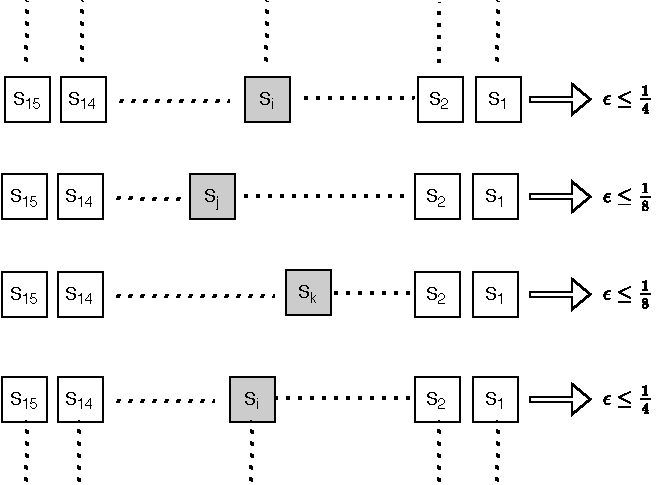
\includegraphics[width=\linewidth]{LC.pdf}
        \endminipage
        \caption{Bias Calculation}
    \end{figure}
    Thus, the bias of this case is bounded by (using pilling up lemma): 
    \begin{equation*}
        \epsilon_4^{(4)} \leq 2^{4-1} \times (2^{-2})^2 \times (2^{-3})^2
    \end{equation*}
    \begin{equation*}
        \epsilon_4^{(4)} \leq 2^{-7} 
    \end{equation*}
    \item Let the number of S-boxes involved over the 4 rounds are 5. Then, the pattern of the active S-boxes cannot be $1-2-1-1$ or $1-1-2-1$. From the above observations, about the S-box we know that, since, the two active S-boxes are initiated by same S-box in the prev. round, therefore they must belong two different sets. Hence, they will activate at least two S-box in the next round. Therefore, the possible pattern for this case is 2-1-1-1 or 1-1-1-2 and hence the bias is bounded by : 
    \begin{equation*}
        \epsilon_4^{(5)} \leq 2^{5-1} \times (2^{-2})^4 \times (2^{-3})
    \end{equation*}
    \begin{equation*}
        \epsilon_4^{(5)} \leq 2^{-7} 
    \end{equation*}
    \item Let the number of active S-boxes is more than 5. In this case, the maximum bias for each round is $\frac{1}{4}$. Therefore, we have : 
    \begin{equation*}
        \epsilon_4^{(i)} \leq 2^{i-1} \times (2^{-2})^i \;\; for \;\; i > 5
    \end{equation*}
    Clearly, the bias is equal to $2^{-7}$ for $i = 6$ and for $i > 6$, the bias is strictly less that $2^{-7}$. 
\end{enumerate}
Thus, from the above analysis, we can conclude that the bias of 4-rounds of linear approximation of present is bounded by $2^{-7}$, that is, $\epsilon_4 \leq 2^{-7}$. Now, we can use this result to bound the linear approximation bias for 28 rounds of PRESENT, which is :
\begin{equation*}
    \epsilon_{28} \leq 2^{6} \times \epsilon_4^{7} = 2^6 \times (2^{-7})^7 \implies \epsilon_{28} \leq 2^{-43}
\end{equation*}
Even for single bit recovery, a good estimate for the number of known plain-texts (N) required for a successful attack is given by : $N = c|\epsilon|^{-2}$, where constant $c \geq 2$. Thus, to attack 31 rounds of PRESENT, the attacker will have to approximate 28 rounds of PRESENT, which will require an order of $2^{86}$ known plain-texts. This, even exceeds the available space which is $2^{64}$. 
\subsection{Correlation Analysis \textsuperscript{\cite{7} \cite{9}}}
In this section, we aim to find whether there exists some reasonable correlation between the encryption time of PRESENT algorithm and the number of set bits in the key. We generate random messages of 64 bit and corresponding to each message we generate random keys with number of set bits varying from 1 to 79.
\begin{figure}[h!]
\minipage{0.45\textwidth}
  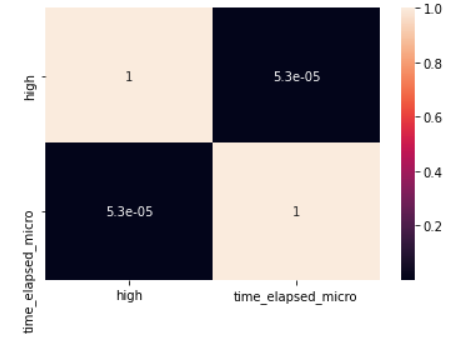
\includegraphics[width=\linewidth]{heatmap.PNG}
\endminipage\hfill
\minipage{0.45\textwidth}
  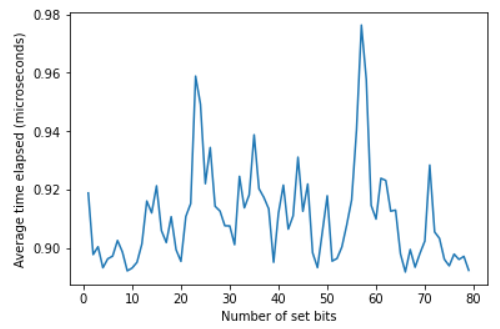
\includegraphics[width=\linewidth]{lineplot.PNG}
\endminipage
\caption{Heatmap and line plot of encryption time vs count of set bits in key}
\end{figure}
From the heatmap, the correlation coefficient is $5.3 \times 10^{-5}$ i.e. very close to zero. A near-zero correlation between the encryption time and number of set bits in key implies that there is no linear relationship between them. Also, from the line plot for number of set bits vs encryption time, we can say that there is no linear relationship between the two variables (or a very weak linear relationship).
\section{Conclusions}
In this paper, we have discussed the design choices of the PRESENT Cipher, including implementation of the cipher and the interesting properties of the S-box, which ensures that the full round PRESENT is resistant to differential and linear attacks. We then analysed a theoretical differential attack of the 16-rounds of the PRESENT cipher and we also implemented 3-Round differential attack of the cipher in python. We then proved that the cipher is resistant to linear cryptanalysis. And at the end, we presented a very interesting experiment, where we tried to analyse side channel characteristics of PRESENT that could affect the run time of encryption function. We believe that, this experiment should be further experimented and we strongly encourage further analysis of the cipher. 
\section{Brownie Point Nomination}
\begin{enumerate}
    \item Correlation analysis : We experimented on various side-channel characteristics of PRESENT that could affect the run time of encryption function. Although on initial experimentation, we found some correlation between number of bits high in the key and the time taken for encryption. But, on randomising the messages also, we could not find any effective correlation. We believe that, this should be further experimented, as there are no paper available on this topic.
    \item Implementation of DC of Reduced Round PRESENT Cipher : We could not find any implementation of Differential analysis on the round reduced version of PRESENT. So, using the idea of differential and filtering taught in the course, we have implemented a differential attack on 3 Rounds of PRESENT. 
\end{enumerate}

\medskip
\printbibliography[title={References}] 
\pagebreak
\begin{center}
    \Large{\textbf{Appendix}}
\end{center}
In this section we discuss the 128-bit key schedule algorithm. Firstly, the initial 128-bit key is stored in a key register $K$ and is represented as $K = k_{127}k_{126}$..$k_0$. At any round $i$, PRESENT extracts the 64-bits round key $K_i = \mathrm{k_{63}}\mathrm{k_{62}}$..$\mathrm{k_{0s}}$ from the current Key (left most 64 bits) register as follows : 
\begin{equation*}
    K_i = \mathrm{k_{63}}\mathrm{k_{62}}..\mathrm{k_{0s}} = k_{127}k_{126}..k_{64}
\end{equation*}
After round key extraction, the key register $K$ is updated according to the following rules : 
\begin{enumerate}
    \item The contents of the key register $K$ is rotated by 61-bits to the left.
    \begin{equation*}
        [k_{127}k_{126}..k_{0}] = [k_{66}k_{67}..k_{68}k_{67}]
    \end{equation*}
    \item The 8-leftmost bits of the key register $K$ is passed through two PRESENT S-boxes.
    \begin{equation*}
        [k_{127}k_{126}k_{125}k_{124}] = S[k_{127}k_{126}k_{125}k_{124}]
    \end{equation*}
    \begin{equation*}
        [k_{123}k_{122}k_{121}k_{120}] = S[k_{123}k_{122}k_{121}k_{120}]
    \end{equation*}
        
    
    \item The 5-bits of key register $k$, $k_{66}k_{65}k_{64}k_{63}k_{62}$ is exclusive-ored with the least significant bits of the round counter value $i$. 
    \begin{equation*}
        [k_{66}k_{65}k_{64}k_{63}k_{62}] = [k_{66}k_{65}k_{64}k_{63}k_{62}] \oplus round-counter
    \end{equation*}
\end{enumerate}

%%%% 8. BILBIOGRAPHY %%%%

% \bibliographystyle{alpha}
% \bibliography{abbrev3,crypto,biblio}
%%%% NOTES
% - Download abbrev3.bib and crypto.bib from https://cryptobib.di.ens.fr/
% - Use bilbio.bib for additional references not in the cryptobib database.
%   If possible, take them from DBLP.




\end{document}
